\documentclass{beamer}
\usepackage{marvosym}
\usepackage{amsfonts,amsmath,amssymb,amsthm, mathtools}
\usepackage[ngerman]{babel}
\usepackage[T1]{fontenc}
\usepackage[utf8]{inputenc}
\usepackage[german]{alg}
\usepackage{tikz, pgf}
\usepackage[font=scriptsize,labelfont=bf]{caption}
\usepackage{verbatim}
\usepackage{comment}
\usetikzlibrary{arrows,shapes}

\pgfdeclarelayer{background}
\pgfsetlayers{background,main}

\theoremstyle{definition}
\newtheorem{korollar}{Korollar}

\mode<presentation>
{
  \usetheme{Ilmenau}
  \usecolortheme{beaver}
  \usefonttheme{professionalfonts}
%  \setbeamercolor{palette primary}{fg=white,bg=black}
  \setbeamercovered{transparent=0}
  \setbeamertemplate{navigation symbols}{}%remove navigation symbols
}
\author{Amelie Koch und Josua Kugler}
\title{Travelling Salesman Problem}
\date{CdE Cyberaka 2020}

\begin{document}
\tikzstyle{vertex}=[circle,fill=black!25,minimum size=20pt,inner sep=0pt, draw = none]
\tikzstyle{selected vertex} = [vertex, fill=red!24, draw = none]
\tikzstyle{edge} = [draw,thick,-]
\tikzstyle{selected edge} = [draw,-,red!50,line width=5pt]
\graphicspath{{images/}}
\maketitle
\begin{frame}
	\frametitle{Motivation}
	\only<1,2,4,6> {
		\begin{itemize}
			\item<1-> Kürzeste Rundreise finden.
			      \begin{itemize}
				      \item<2-> 	Handlungsreisende
				      \item<4-> 	Computerchips
			      \end{itemize}
		\end{itemize}}
	\only<3> {
		\begin{figure}
			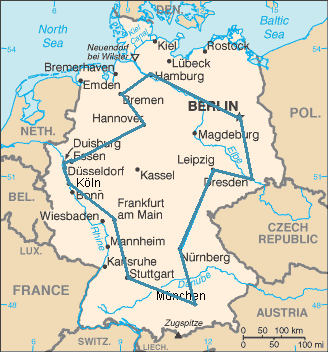
\includegraphics[scale=0.4]{images/TSP_Deutschland_3.png}
			\caption{Optimaler Reiseweg eines Handlungsreisenden durch die 15 größten Städte Deutschlands. Die angegebene Route ist die kürzeste von 43.589.145.600 möglichen.}
		\end{figure}
	}
	\only<5>{
		\begin{figure}
			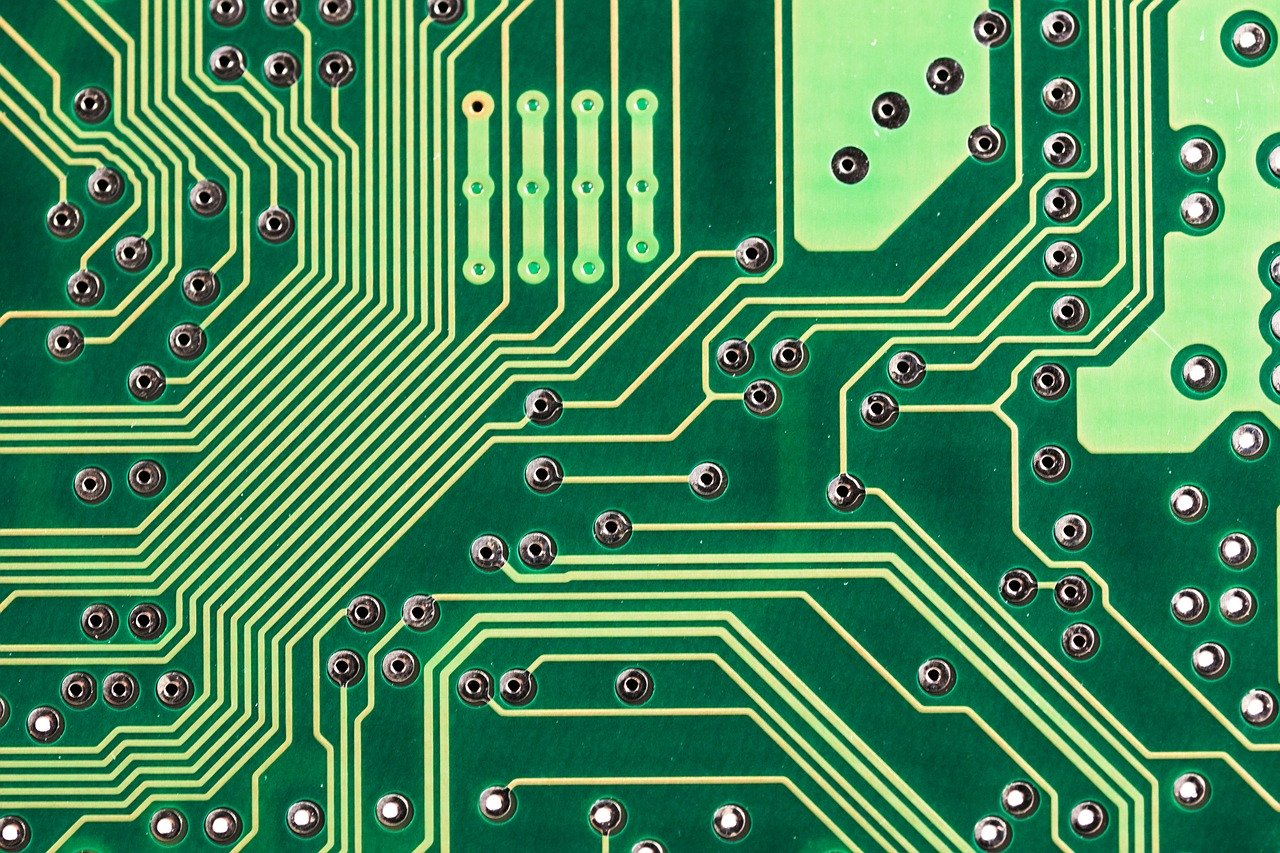
\includegraphics[scale=0.17]{images/computer-chip.jpg}
			\caption{Ein großer Teil des Aufwands beim Erstellen vom Computerchips entfällt auf Optimierung, z.B. auch die kürzeste Route zum Bohren zu finden.}
		\end{figure}
	}
\end{frame}
  \section*{Grundlagen}
  \begin{frame}
    \frametitle{Grundlegende Definitionen}

\begin{columns}
\begin{column}{0.58\textwidth}
    Sei $G = (V,E)$ ein Graph mit Knotenmenge $V$ und Kantenmenge $E$.
    \only<2>{
    \begin{definition}[Pfad]
                %Ein \textbf{Pfad} der Länge $n$ ist eine Folge von paarweise verschiedenen Knoten $(v_0, v_1, \dots, v_n) \in V^n$, sodass Kanten $e = (v_i-1, v_i)\in E\quad \forall 1 \leq i \leq n$ existieren.
                $v_0, v_1, \dots, v_n \in V$ mit Kanten $e = (v_{i-1}, v_i)\in E\quad \forall 1 \leq i \leq n$
    \end{definition}
    }
    \only<3->{
    \begin{definition}[zusammenhängend]
        $\forall v_1, v_2 \in V \exists$ Pfad von $v_1$ nach $v_2$.
    \end{definition}
    \begin{definition}[Zusammenhangskomponenten]
        maximal zusammenhängende Teilgraphen
    \end{definition}
    }
\end{column}
\begin{column}{0.43\textwidth}
    \only<1> {
    \begin{figure}
        \begin{tikzpicture}[scale=1.3, auto,swap]
            % Draw a 7,11 network
            % First we draw the vertices
            \foreach \pos/\name in {{(0,0)/a}, {(1,1)/b}, {(3,1)/c},
            {(0,-2)/d}, {(2,0)/e}, {(1,-1)/f}, {(3,-1)/g}}
            \node[vertex] (\name) at \pos {$\name$};
            % Connect vertices with edges and draw weights
            \foreach \source/ \dest /\weight in {b/a/1, c/b/2,d/a/4,d/b/2,
            e/b/3, e/c/5, d/g/2,
            f/d/4,f/e/1,
            g/e/3,g/f/5}
            \path[edge] (\source) -- node[font=\small] {} (\dest);
        \end{tikzpicture}
    \end{figure}
    }
    \only<2> {
    \begin{figure}
        \begin{tikzpicture}[scale=1.3, auto,swap]
            % Draw a 7,11 network
            % First we draw the vertices
            \foreach \pos/\name in {{(0,0)/a}, {(1,1)/b}, {(3,1)/c},
            {(0,-2)/d}, {(2,0)/e}, {(1,-1)/f}, {(3,-1)/g}}
            \node[vertex] (\name) at \pos {$\name$};
            % Connect vertices with edges and draw weights
            \foreach \source/ \dest /\weight in {b/a/1, c/b/2,d/a/4,d/b/2,
            e/b/3, e/c/5, d/g/2,
            f/d/4,f/e/1,
            g/e/3,g/f/5}
            \path[edge] (\source) -- node[font=\small] {} (\dest);
            
            \begin{pgfonlayer}{background}
            \foreach \source / \dest in {b/a,c/b,c/e,e/g,g/d}
            \path[selected edge] (\source.center) -- (\dest.center);
            \end{pgfonlayer}
        \end{tikzpicture}
	\end{figure}
    }
    \only<3> {
    \begin{figure}
        \begin{tikzpicture}[scale=1.3, auto,swap]
            % Draw a 7,11 network
            % First we draw the vertices
            \foreach \pos/\name in {{(0,0)/a}, {(1,1)/b}, {(3,1)/c},
            {(0,-2)/d}, {(2,0)/e}, {(1,-1)/f}, {(3,-1)/g}}
            \node[vertex] (\name) at \pos {$\name$};
            % Connect vertices with edges and draw weights
            \foreach \source/ \dest /\weight in {b/a/1,d/a/4,d/b/2,
            e/b/3,  d/g/2,
            f/d/4,f/e/1,
            g/e/3,g/f/5}
            \path[edge] (\source) -- node[font=\small] {} (\dest);
        \end{tikzpicture}
    \end{figure}
    }
    \only<4> {
    \begin{figure}
        \begin{tikzpicture}[scale=1.3, auto,swap]
            % Draw a 7,11 network
            % First we draw the vertices
            \foreach \pos/\name in {{(0,0)/a}, {(1,1)/b}, 
            {(0,-2)/d}, {(2,0)/e}, {(1,-1)/f}, {(3,-1)/g}}
            \node[vertex] (\name) at \pos {$\name$};
            % Connect vertices with edges and draw weights
            \foreach \source/ \dest /\weight in {b/a/1,d/a/4,d/b/2,
            e/b/3,  d/g/2,
            f/d/4,f/e/1,
            g/e/3,g/f/5}
            \path[edge] (\source) -- node[font=\small] {} (\dest);
        \end{tikzpicture}
    \end{figure}
    }
    \end{column}
\end{columns}
\end{frame}
  \begin{frame}
    \frametitle{Grundlegende Definitionen}

\begin{columns}
\begin{column}{0.58\textwidth}

\only<1-3> {
    \begin{definition}[Kreis]
        Ist $(v_1, \dots, v_{n-1})$ mit $n > 1$ ein Pfad, so heißt $(v_0, \dots, v_{n-1}, v_0)$ Kreis.
    \end{definition}
}
\only<3>{
    \begin{definition}
        Einen Graphen ohne Kreise nennt man \textbf{azyklisch}.
    \end{definition}
}

\only<4->{
    \begin{definition}[Grad]
        %Sei $v\in V$ ein Knoten in einem Graphen $G = (V,E)$. Dann heißt $\# \{e \in E| v \in e\}$ der Grad von $v$.
        $d(v) = |\{e \in E| v \in e\}|$
    \end{definition}
    \begin{lemma}
        Die Anzahl der Knoten mit ungeradem Grad ist gerade.
    \end{lemma}
}

\end{column}
\begin{column}{0.43\textwidth}

    \only<1> {
    \begin{figure}
        \begin{tikzpicture}[scale=1.3, auto,swap]
        % First we draw the vertices
        \foreach \pos/\name in {{(0,2)/a}, {(0,0)/b}, {(1,-1)/c},
                                {(2,0)/d}, {(2,2)/e}}
        \node[vertex] (\name) at \pos {$\name$};
        % Connect vertices with edges and draw weights
        \foreach \source/ \dest /\weight in {b/a/1, c/b/2,
                                            c/d/3, d/e/5, e/a/6}
        \path[edge] (\source) -- node[font=\small] {} (\dest);
        \end{tikzpicture}
    \end{figure}
    }

    \only<2> {
    \begin{figure}
        \begin{tikzpicture}[scale=1.3, auto,swap]
        % Draw a 7,11 network
        % First we draw the vertices
        \foreach \pos/\name in {{(0,2)/a}, {(0,0)/b}, {(1,-1)/c},
                                {(2,0)/d}, {(2,2)/e}}
            \node[vertex] (\name) at \pos {$\name$};
        % Connect vertices with edges and draw weights
        \foreach \source/ \dest /\weight in {b/a/1, c/b/2,
                                            c/d/3, d/e/5, e/a/6}
            \path[edge] (\source) -- node[font=\small] {} (\dest);
            \begin{pgfonlayer}{background}
                \foreach \source / \dest in {b/a,c/b,d/c,d/e,e/a}
                \path[selected edge] (\source.center) -- (\dest.center);   
            \end{pgfonlayer}
        \end{tikzpicture}
    \end{figure}
    }

    

\only<3> {
\begin{figure}
		\begin{tikzpicture}[scale=1.3, auto,swap]
    % Draw a 7,11 network
    % First we draw the vertices
    \foreach \pos/\name in {{(0,2)/a}, {(0,0)/b}, {(1,-1)/c},
                            {(2,0)/d}, {(2,2)/e}}
        \node[vertex] (\name) at \pos {$\name$};
    % Connect vertices with edges and draw weights
    \foreach \source/ \dest /\weight in {b/a/1, c/b/2,
                                         c/d/3, d/e/5}
        \path[edge] (\source) -- node[font=\small] {} (\dest);
    
		\end{tikzpicture}
\end{figure}
}

\only<4>{
\begin{figure}
		\begin{tikzpicture}[scale=1.3, auto,swap]
    % Draw a 7,11 network
    % First we draw the vertices
    \foreach \pos/\name in {{(0,0)/a}, {(1,1)/b}, {(3,1)/c},
                            {(0,-2)/d}, {(2,0)/e}, {(1,-1)/f}, {(3,-1)/g}};
   	\node[vertex] (a) at (0,0) {$2$};
   	\node[vertex] (b) at (1,1) {$4$};
   	\node[vertex] (c) at (3,1) {$2$};
   	\node[vertex] (d) at (0,-2) {$4$};
   	\node[vertex] (e) at (2,0) {$4$};
   	\node[vertex] (f) at (1,-1) {$3$};
   	\node[vertex] (g) at (3,-1) {$3$};
   	
    % Connect vertices with edges and draw weights
    \foreach \source/ \dest /\weight in {b/a/1, c/b/2,d/a/4,d/b/2,
                                         e/b/3, e/c/5, d/g/2,
                                         f/d/4,f/e/1,
                                         g/e/3,g/f/5}
        \path[edge] (\source) -- node[font=\small] {} (\dest);
	\end{tikzpicture}
\end{figure}
}
\end{column}
\end{columns}
\end{frame}
  \begin{frame}
\frametitle{Definition Baum}

\begin{columns}
\begin{column}{0.58\textwidth}

\only<1>{
    \begin{definition}
        Ein Baum ist eine ausdauernde und verholzende Samenpflanze mit einer dominierende Sprossachse, die durch sekundäres Dickenwachstum an Umfang zunimmt.
    \end{definition}
}
\only<2>{Nein Spass, jedes Kind weiß, dass das so nicht stimmt. In Wirklichkeit ist das ganz anders.}
\only<3->{
    \begin{definition}[Baum]
        %Ein \textbf{Baum} ist ein zusammenhängender, azyklischer Graph. Ein Graph, dessen Zusammenhangskomponenten Bäume sind, heißt \textbf{Wald}.
        zusammenhängender, azyklischer Graph
    \end{definition}
}
\only<4>{
    \begin{definition}[Wald]
        Graph, dessen Zusammenhangskomponenten Bäume sind
    \end{definition}
}
\only<5>{
    \begin{definition}[aufspannender Baum]
        Ein \textbf{aufspannender Baum} eines Graphen $G$ ist ein Baum, der alle Knoten von $G$ enthält.
    \end{definition}
}
\only<6>{
    \begin{definition}[Blatt]
        Ein Knoten eines Baums mit Grad 1 heißt \textbf{Blatt}.
    \end{definition}
}
\end{column}
\begin{column}{0.43\textwidth}
\only<1>{
\begin{figure}
    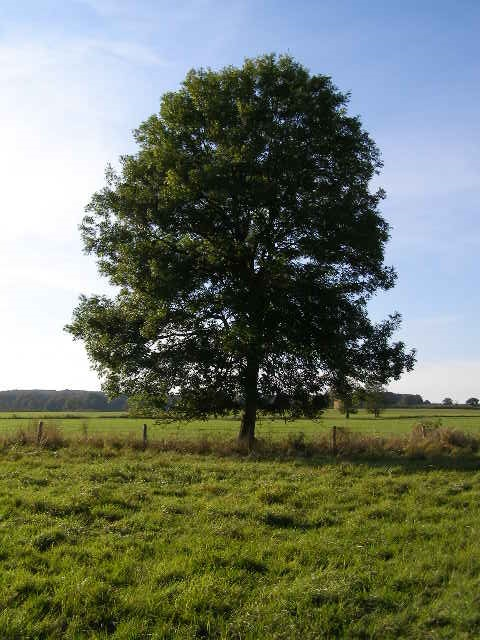
\includegraphics[width= \textwidth]{baum.jpg}
\end{figure}
}
\only<3> {
	\begin{figure}
		\begin{tikzpicture}[scale=1.3, auto,swap]
    % Draw a 7,11 network
    % First we draw the vertices
    \foreach \pos/\name in {{(0,0)/a}, {(1,1)/b}, {(3,1)/c},
                            {(0,-2)/d}, {(2,0)/e}, {(1,-1)/f}, {(3,-1)/g}}
        \node[vertex] (\name) at \pos {$\name$};
    % Connect vertices with edges and draw weights
    \foreach \source/ \dest /\weight in {b/a/1, c/b/2,d/a/4,
                                         e/b/3,
                                         f/d/4,
                                         g/e/3}
        \path[edge] (\source) -- node[font=\small] {} (\dest);
    
        
	\end{tikzpicture}
	\end{figure}
}
\only<4> {
	\begin{figure}
		\begin{tikzpicture}[scale=1.3, auto,swap]
    % Draw a 7,11 network
    % First we draw the vertices
    \foreach \pos/\name in {{(0,0)/a}, {(1,1)/b}, {(3,1)/c},
                            {(0,-2)/d}, {(2,0)/e}, {(1,-1)/f}, {(3,-1)/g}}
        \node[vertex] (\name) at \pos {$\name$};
    % Connect vertices with edges and draw weights
    \foreach \source/ \dest /\weight in {c/b/2,d/a/4,
                                         e/b/3,
                                         f/d/4,
                                         g/e/3}
        \path[edge] (\source) -- node[font=\small] {} (\dest);
    
        
	\end{tikzpicture}
	\end{figure}
}
\only<5>{
	\begin{figure}
		\begin{tikzpicture}[scale=1.3, auto,swap]
    % Draw a 7,11 network
    % First we draw the vertices
    \foreach \pos/\name in {{(0,0)/a}, {(1,1)/b}, {(3,1)/c},
                            {(0,-2)/d}, {(2,0)/e}, {(1,-1)/f}, {(3,-1)/g}}
        \node[vertex] (\name) at \pos {$\name$};
    % Connect vertices with edges and draw weights
    \foreach \source/ \dest /\weight in {b/a/1, c/b/2,d/a/4,d/b/2,
                                         e/b/3, e/c/5, d/g/2,
                                         f/d/4,f/e/1,
                                         g/e/3,g/f/5}
        \path[edge] (\source) -- node[font=\small] {} (\dest);
    
     \begin{pgfonlayer}{background}
        \foreach \source / \dest in {b/a,c/b,d/a,e/b,f/d,g/e}
            \path[selected edge] (\source.center) -- (\dest.center);
            
    \end{pgfonlayer}
\end{tikzpicture}
	\end{figure}
}
\only<6> {
	\begin{figure}
		\begin{tikzpicture}[scale=1.3, auto,swap]
        \foreach \pos/\name in {{(0,0)/a}, {(1,1)/b},
                                {(0,-2)/d}, {(2,0)/e}}
            \node[vertex] (\name) at \pos {$\name$};
        \foreach \pos/\name in {{(3,1)/c},
            {(1,-1)/f}, {(3,-1)/g}}
            \node[selected vertex] (\name) at \pos {$\name$};
        % Connect vertices with edges and draw weights
        \foreach \source/ \dest /\weight in {c/b/2,d/a/4, a/b/1, b/e/1
                                            e/b/3,
                                            f/d/4,
                                            g/e/3}
            \path[edge] (\source) -- node[font=\small] {} (\dest);
	\end{tikzpicture}
	\end{figure}
}
\end{column}
\end{columns}
\end{frame}
  \begin{frame}[t]
\frametitle{Grundlegende Eigenschaften eines Baums}
\begin{lemma}
    In einem Baum gibt es genau einen Pfad zwischen zwei Knoten.
\end{lemma}

\only<2->{
\begin{proof}
    \vspace*{-0.6cm}
}%
\begin{columns}
    \begin{column}{0.58\textwidth}
        \begin{itemize}
            \item<2-> Zusammenhang $\implies \exists$ Pfad.
            \item<4-> Annahme: Es gibt verschiedene Pfade zwischen $v_1$ und $v_2$ $\implies$ Kreis $\implies$ \Lightning.
        \end{itemize}
    \end{column}
    \begin{column}{0.25\textwidth}
        \only<2> {
            \begin{figure}
                \begin{tikzpicture}[scale=1, auto,swap]
                \foreach \pos/\name in {{(0,0)/a}, {(1,1)/b}, {(3,1)/c},{(0,-2)/d}, {(2,0)/e}, {(1,-1)/f}, {(3,-1)/g}} \node[vertex] (\name) at \pos {$\name$};
                \foreach \source/ \dest /\weight in {b/a/1, c/b/2,d/a/4,e/b/3,f/d/4,g/e/3}
                    \path[edge] (\source) -- (\dest);
                \end{tikzpicture}
            \end{figure}
        }
        \only<3> {
            \begin{figure}
                \begin{tikzpicture}[scale=1, auto,swap]
                % Draw a 7,11 network
                % First we draw the vertices
                \foreach \pos/\name in {{(0,0)/a}, {(1,1)/b}, {(3,1)/c},
                                        {(0,-2)/d}, {(2,0)/e}, {(1,-1)/f}, {(3,-1)/g}}
                    \node[vertex] (\name) at \pos {$\name$};
                \foreach \source/ \dest /\weight in {b/a/1, d/a/4,e/b/3,f/d/4,g/e/3}
                    \path[edge] (\source) -- node[font=\small] {} (\dest);
                \end{tikzpicture}
            \end{figure}
        }
        \only<4>{
            \vspace*{0.1mm}
            \begin{figure}
                    \begin{tikzpicture}[scale=1, auto,swap]
                % Draw a 7,11 network
                % First we draw the vertices
                \foreach \pos/\name in {{(0,1)/a}, {(0,0)/b}, {(1,-1)/c},
                                        {(2,0)/d}, {(2,1)/e}, {(1,2)/f}}
                    \node[vertex] (\name) at \pos {$\name$};
                % Connect vertices with edges and draw weights
                \foreach \source/ \dest /\weight in {b/a/1, c/b/2,
                                                     c/d/3, d/e/5, a/f/1, f/e/1}
                    \path[edge] (\source) -- node[font=\small] {} (\dest);
                
                    \end{tikzpicture}
            \end{figure}
            }
            \only<5> {
            \vspace*{0.1mm}
            \begin{figure}
                    \begin{tikzpicture}[scale=1, auto,swap]
                % Draw a 7,11 network
                % First we draw the vertices
                \foreach \pos/\name in {{(0,1)/a}, {(0,0)/b}, {(1,-1)/c},
                                        {(2,0)/d}, {(2,1)/e}, {(1,2)/f}}
                    \node[vertex] (\name) at \pos {$\name$};
                % Connect vertices with edges and draw weights
                \foreach \source/ \dest /\weight in {b/a/1, c/b/2,
                                                     c/d/3, d/e/5, a/f/1, f/e/1}
                    \path[edge] (\source) -- node[font=\small] {} (\dest);
                        
                \begin{pgfonlayer}{background}
                    \foreach \source / \dest in {b/a,c/b,f/a}
                        \path[selected edge] (\source.center) -- (\dest.center);
                        
                \end{pgfonlayer}
                    \end{tikzpicture}
            \end{figure}
            }
            \only<6> {
            \vspace*{0.1mm}
            \begin{figure}
                    \begin{tikzpicture}[scale=1, auto,swap]
                % Draw a 7,11 network
                % First we draw the vertices
                \foreach \pos/\name in {{(0,1)/a}, {(0,0)/b}, {(1,-1)/c},
                                        {(2,0)/d}, {(2,1)/e}, {(1,2)/f}}
                    \node[vertex] (\name) at \pos {$\name$};
                % Connect vertices with edges and draw weights
                \foreach \source/ \dest /\weight in {b/a/1, c/b/2,
                                                     c/d/3, d/e/5, a/f/1, f/e/1}
                    \path[edge] (\source) -- node[font=\small] {} (\dest);
                        
                \begin{pgfonlayer}{background}
                    \foreach \source / \dest in {f/e,e/d,d/c}
                        \path[selected edge] (\source.center) -- (\dest.center);
                        
                \end{pgfonlayer}
                    \end{tikzpicture}
            \end{figure}    
            }
            \only<7> {
                \vspace*{0.1mm}
                \begin{figure}
                        \begin{tikzpicture}[scale=1, auto,swap]
                    % Draw a 7,11 network
                    % First we draw the vertices
                    \foreach \pos/\name in {{(0,1)/a}, {(0,0)/b}, {(1,-1)/c},
                                            {(2,0)/d}, {(2,1)/e}, {(1,2)/f}}
                        \node[vertex] (\name) at \pos {$\name$};
                    % Connect vertices with edges and draw weights
                    \foreach \source/ \dest /\weight in {b/a/1, c/b/2,
                                                         c/d/3, d/e/5, a/f/1, f/e/1}
                        \path[edge] (\source) -- node[font=\small] {} (\dest);
                            
                    \begin{pgfonlayer}{background}
                        \foreach \source / \dest in {f/e,e/d,d/c,b/a,c/b,f/a}
                            \path[selected edge] (\source.center) -- (\dest.center);
                            
                    \end{pgfonlayer}
                        \end{tikzpicture}
                \end{figure}
                }           
    \end{column}
    \begin{column}{0.13\textwidth}
        \hspace*{2cm}
    \end{column}
\end{columns}
\only<2->{
\end{proof}
}
\end{frame}
  \begin{frame}[t]
\frametitle{Grundlegende Eigenschaften eines Baums}
\begin{lemma}
        Ein Baum ist minimal zusammenhängend und maximal kreisfrei.
\end{lemma}
\only<2->{
\begin{proof}
    \vspace*{-0.6cm}
}%
\begin{columns}
    \begin{column}{0.58\textwidth}
        \begin{itemize}
            \item<2-> Kante entfernen 
            \begin{itemize}
                \item[$\implies$]<3-> Pfad unterbrochen 
                \item[$\overset{\mathclap{\text{Lemma 1}}}{\implies}$]<4-> nicht mehr zusammenhängend
            \end{itemize}
            \item<5-> Kante hinzufügen 
            \begin{itemize}
                \item[$\implies$]<6-> neuer Weg 
                \item[$\overset{\mathclap{\text{Lemma 1}}}{\implies}$]<7-> Kreis
            \end{itemize}
        \end{itemize}
    \end{column}
    \begin{column}{0.25\textwidth}
        \only<2> {
        \begin{figure}
                \begin{tikzpicture}[scale=1, auto,swap]
            % Draw a 7,11 network
            % First we draw the vertices
            \foreach \pos/\name in {{(0,2)/a}, {(0,0)/b}, {(1,-1)/c},
                                    {(2,0)/d}, {(2,2)/e}}
                \node[vertex] (\name) at \pos {$\name$};
            % Connect vertices with edges and draw weights
            \foreach \source/ \dest /\weight in {b/a/1, c/b/2,
                                                c/d/3, d/e/5}
                \path[edge] (\source) -- node[font=\small] {} (\dest);
            
                \end{tikzpicture}
        \end{figure}
        }

        \only<3-4> {
        \begin{figure}
                \begin{tikzpicture}[scale=1, auto,swap]
            % Draw a 7,11 network
            % First we draw the vertices
            \foreach \pos/\name in {{(0,2)/a}, {(0,0)/b}, {(1,-1)/c},
                                    {(2,0)/d}, {(2,2)/e}}
                \node[vertex] (\name) at \pos {$\name$};
            % Connect vertices with edges and draw weights
            \foreach \source/ \dest /\weight in {b/a/1, c/b/2,
                                                d/e/5}
                \path[edge] (\source) -- node[font=\small] {} (\dest);
            
                \end{tikzpicture}
        \end{figure}
        }

        \only<5> {
        \begin{figure}
                \begin{tikzpicture}[scale=1, auto,swap]
            % Draw a 7,11 network
            % First we draw the vertices
            \foreach \pos/\name in {{(0,2)/a}, {(0,0)/b}, {(1,-1)/c},
                                    {(2,0)/d}, {(2,2)/e}}
                \node[vertex] (\name) at \pos {$\name$};
            % Connect vertices with edges and draw weights
            \foreach \source/ \dest /\weight in {b/a/1, c/b/2,
                                                c/d/3, d/e/5}
                \path[edge] (\source) -- node[font=\small] {} (\dest);
            
                \end{tikzpicture}
        \end{figure}
        }
        \only<6> {
        \begin{figure}
                \begin{tikzpicture}[scale=1, auto,swap]
            % Draw a 7,11 network
            % First we draw the vertices
            \foreach \pos/\name in {{(0,2)/a}, {(0,0)/b}, {(1,-1)/c},
                                    {(2,0)/d}, {(2,2)/e}}
                \node[vertex] (\name) at \pos {$\name$};
            % Connect vertices with edges and draw weights
            \foreach \source/ \dest /\weight in {b/a/1, c/b/2,
                                                c/d/3, d/e/5,a/e/1}
                \path[edge] (\source) -- node[font=\small] {} (\dest);
            
                \end{tikzpicture}
        \end{figure}
        }
        \only<7> {
        \begin{figure}
                \begin{tikzpicture}[scale=1, auto,swap]
            % Draw a 7,11 network
            % First we draw the vertices
            \foreach \pos/\name in {{(0,2)/a}, {(0,0)/b}, {(1,-1)/c},
                                    {(2,0)/d}, {(2,2)/e}}
                \node[vertex] (\name) at \pos {$\name$};
            % Connect vertices with edges and draw weights
            \foreach \source/ \dest /\weight in {b/a/1, c/b/2,
                                                c/d/3, d/e/5, e/a/6}
                \path[edge] (\source) -- node[font=\small] {} (\dest);
            
            \begin{pgfonlayer}{background}
                \foreach \source / \dest in {b/a,c/b,d/c,d/e,e/a}
                    \path[selected edge] (\source.center) -- (\dest.center);
                    
            \end{pgfonlayer}
                \end{tikzpicture}
        \end{figure}
        }
    \end{column}
\begin{column}{0.13\textwidth}
    \hspace*{2cm}
\end{column}
\end{columns}
\only<2->{
\end{proof}
}
\end{frame}
  \begin{frame}[t]
\frametitle{Grundlegende Eigenschaften eines Baums}
\only<5>{%
\begin{lemma}%
In einem Baum gibt es genau einen Pfad zwischen zwei Knoten.%
\end{lemma}%
\begin{lemma}%
Ein Baum ist minimal zusammenhängend und maximal kreisfrei.%
\end{lemma}%
}%
\begin{lemma}
        Ein Baum mit $n$ Knoten besitzt $n-1$ Kanten.
\end{lemma}
\only<2-4>{
\begin{proof}
}%
\begin{columns}
    \begin{column}{0.58\textwidth}
            \begin{itemize}
                \item<2-4> Induktionsanfang:\\ 1 Knoten $\implies$ 0 Kanten
                \item<3-4> Induktionsschritt:\\
                $k \to k +1$ Knoten $\implies + 1$ Kante, sonst Kreis.
            \end{itemize} 
    \end{column}
    \begin{column}{0.25\textwidth}
        \only<2>{
            \begin{figure}
                \begin{tikzpicture}[scale=1, auto,swap]
                    \node[vertex] (a) at (0,0) {$a$};
                \end{tikzpicture}
        \end{figure}
        }
        \only<3>{\vspace*{-0.4cm}
            \begin{figure}
                \begin{tikzpicture}[scale=1, auto,swap]
            % Draw a 7,11 network
            % First we draw the vertices
            \foreach \pos/\name in {{(0,2)/a}, {(0,0)/b}, {(1,-1)/c},
                                    {(2,0)/d}, {(2,2)/e}}
                \node[vertex] (\name) at \pos {$\name$};
            % Connect vertices with edges and draw weights
            \foreach \source/ \dest /\weight in {b/a/1, c/b/2,
                                                c/d/3}
                \path[edge] (\source) -- node[font=\small] {} (\dest);
            
                \end{tikzpicture}
        \end{figure}
        }
        \only<4>{\vspace*{-0.4cm}
            \begin{figure}
                \begin{tikzpicture}[scale=1, auto,swap]
            % Draw a 7,11 network
            % First we draw the vertices
            \foreach \pos/\name in {{(0,2)/a}, {(0,0)/b}, {(1,-1)/c},
                                    {(2,0)/d}, {(2,2)/e}}
                \node[vertex] (\name) at \pos {$\name$};
            % Connect vertices with edges and draw weights
            \foreach \source/ \dest /\weight in {b/a/1, c/b/2,
                                                c/d/3, d/e/5}
                \path[edge] (\source) -- node[font=\small] {} (\dest);
            
                \end{tikzpicture}
        \end{figure}
        }
    \end{column}
    \begin{column}{0.13\textwidth}
        \hspace*{2cm}
    \end{column}
\end{columns}
\only<2-4>{
\end{proof}
}
\end{frame}
  \begin{frame}

\frametitle{Definition Baum}

    \frametitle{Allgemeine Definitionen}
\only<1,3>{
    \begin{definition}
        Ein Graph $G = (V,E)$ mit einer Funktion $w: E \to \mathbb{R}$ heißt gewichteter Graph.
    \end{definition}
}
\only<2> {
	\begin{figure}
		\begin{tikzpicture}[scale=1.8, auto,swap]
    % Draw a 7,11 network
    % First we draw the vertices
    \foreach \pos/\name in {{(0,0)/a}, {(1,1)/b}, {(3,1)/c},
                            {(0,-2)/d}, {(2,0)/e}, {(1,-1)/f}, {(3,-1)/g}}
        \node[vertex] (\name) at \pos {$\name$};
    % Connect vertices with edges and draw weights
    \foreach \source/ \dest /\weight in {b/a/1, c/b/2,d/a/4,
                                         e/b/3,
                                         f/d/4,
                                         g/e/3}
        \path[edge] (\source) -- node[font=\small] {$\weight$} (\dest);
    
        
	\end{tikzpicture}
	\end{figure}
}
\only<3>{
    \begin{definition}
        Der minimale Spannbaum $G' = (V, E')$ eines gewichteten, zusammenhängenden Graphen $G = (V,E)$ ist ein aufspannender Baum, für den \[\sum_{e \in E'} w(e)\] minimal ist.
    \end{definition}
}
\only<4>{
	\begin{figure}
		\begin{tikzpicture}[scale=1.8, auto,swap]
    % Draw a 7,11 network
    % First we draw the vertices
    \foreach \pos/\name in {{(0,0)/a}, {(1,1)/b}, {(3,1)/c},
                            {(0,-2)/d}, {(2,0)/e}, {(1,-1)/f}, {(3,-1)/g}}
        \node[vertex] (\name) at \pos {$\name$};
    % Connect vertices with edges and draw weights
    \foreach \source/ \dest /\weight in {b/a/1, c/b/2,d/a/4,d/b/9,
                                         e/b/3, e/c/42, d/g/15,
                                         f/d/4,f/e/7,
                                         g/e/3,g/f/5}
        \path[edge] (\source) -- node[font=\small] {$\weight$} (\dest);
    
     \begin{pgfonlayer}{background}
        \foreach \source / \dest in {b/a,c/b,d/a,e/b,f/d,g/e}
            \path[selected edge] (\source.center) -- (\dest.center);
            
    \end{pgfonlayer}
\end{tikzpicture}
	\end{figure}
}
\end{frame}
  \section*{Kruskal-Algorithmus}
  \begin{frame}
    \frametitle{Algorithmus von Kruskal}
    \begin{algorithm}
        \alginout{gewichteter Graph $G = (V,E)$, Funktion $w : E \rightarrow \mathbb{R}$  }{minimaler Spannbaum $G'(V, E')$ von $G$}
        \begin{algtab}
            \algwhile{$|E'| < |V| - t$}
            		betrachte Kante $e$ aus $G$ mit $w(e) = \min_{e \in E}w(e)$\\
                    \algifthenelse{$G'$ mit $e$ azyklisch}{$e$ von $G$ zu $G'$}{entferne $e$ in $G$}
        \end{algtab}
    \end{algorithm}
\end{frame}

  %visualizegraphalgorithm("kruskal",
%       "kruskal_plot", 
%       ["a", "b", "c", "d", "e"], 
%       [
%       ("a", "b", 1), 
%       ("b", "c", 2), 
%       ("a", "c", 1), 
%       ("e", "d", 2), 
%       ("a", "e", 3), 
%       ("c", "e", 3),
%       ("e", "a", 5)
%], 0.75)
%END
\begin{frame}
    \begin{columns}[T] % align columns
        \begin{column}{.36\textwidth}
\only<1>{

\begin{tikzpicture}[>=latex,line join=bevel,scale=0.75, auto]
%%
\node (a) at (125.0bp,279.0bp) [draw,ellipse,vertex] {$a$};
  \node (b) at (27.0bp,192.0bp) [draw,ellipse,vertex] {$b$};
  \node (c) at (70.0bp,105.0bp) [draw,ellipse,vertex] {$c$};
  \node (e) at (125.0bp,18.0bp) [draw,ellipse,vertex] {$e$};
  \node (d) at (180.0bp,105.0bp) [draw,ellipse,vertex] {$d$};
  \draw [black,edge] (a) ..controls (92.968bp,261.12bp) and (79.626bp,252.44bp)  .. (69.0bp,243.0bp) .. controls (57.512bp,232.79bp) and (46.543bp,219.29bp)  .. node {$1$} (b);
  \draw [black,edge] (a) ..controls (115.58bp,255.68bp) and (113.09bp,249.09bp)  .. (111.0bp,243.0bp) .. controls (96.429bp,200.44bp) and (82.078bp,149.5bp)  .. node {$1$} (c);
  \draw [black,edge] (a) ..controls (125.0bp,212.73bp) and (125.0bp,84.232bp)  .. node {$5$} (e);
  \draw [black,edge] (b) ..controls (43.034bp,159.56bp) and (53.989bp,137.39bp)  .. node {$2$} (c);
  \draw [black,edge] (c) ..controls (90.344bp,72.82bp) and (104.7bp,50.112bp)  .. node {$3$} (e);
  \draw [black,edge] (d) ..controls (159.66bp,72.82bp) and (145.3bp,50.112bp)  .. node {$2$} (e);
%
\end{tikzpicture}


}
\only<2>{

\begin{tikzpicture}[>=latex,line join=bevel,scale=0.75, auto]
%%
\node (a) at (125.0bp,279.0bp) [draw,ellipse,vertex] {$a$};
  \node (b) at (27.0bp,192.0bp) [draw,ellipse,vertex] {$b$};
  \node (c) at (70.0bp,105.0bp) [draw,ellipse,vertex] {$c$};
  \node (e) at (125.0bp,18.0bp) [draw,ellipse,vertex] {$e$};
  \node (d) at (180.0bp,105.0bp) [draw,ellipse,vertex] {$d$};
  \draw [red,edge] (a) ..controls (92.968bp,261.12bp) and (79.626bp,252.44bp)  .. (69.0bp,243.0bp) .. controls (57.512bp,232.79bp) and (46.543bp,219.29bp)  .. node {$1$} (b);
  \draw [black,edge] (a) ..controls (115.58bp,255.68bp) and (113.09bp,249.09bp)  .. (111.0bp,243.0bp) .. controls (96.429bp,200.44bp) and (82.078bp,149.5bp)  .. node {$1$} (c);
  \draw [black,edge] (a) ..controls (125.0bp,212.73bp) and (125.0bp,84.232bp)  .. node {$5$} (e);
  \draw [black,edge] (b) ..controls (43.034bp,159.56bp) and (53.989bp,137.39bp)  .. node {$2$} (c);
  \draw [black,edge] (c) ..controls (90.344bp,72.82bp) and (104.7bp,50.112bp)  .. node {$3$} (e);
  \draw [black,edge] (d) ..controls (159.66bp,72.82bp) and (145.3bp,50.112bp)  .. node {$2$} (e);
%
\end{tikzpicture}


}
\only<3>{

\begin{tikzpicture}[>=latex,line join=bevel,scale=0.75, auto]
%%
\node (a) at (125.0bp,279.0bp) [draw,ellipse,vertex] {$a$};
  \node (b) at (27.0bp,192.0bp) [draw,ellipse,vertex] {$b$};
  \node (c) at (70.0bp,105.0bp) [draw,ellipse,vertex] {$c$};
  \node (e) at (125.0bp,18.0bp) [draw,ellipse,vertex] {$e$};
  \node (d) at (180.0bp,105.0bp) [draw,ellipse,vertex] {$d$};
  \draw [red,edge] (a) ..controls (92.968bp,261.12bp) and (79.626bp,252.44bp)  .. (69.0bp,243.0bp) .. controls (57.512bp,232.79bp) and (46.543bp,219.29bp)  .. node {$1$} (b);
  \draw [red,edge] (a) ..controls (115.58bp,255.68bp) and (113.09bp,249.09bp)  .. (111.0bp,243.0bp) .. controls (96.429bp,200.44bp) and (82.078bp,149.5bp)  .. node {$1$} (c);
  \draw [black,edge] (a) ..controls (125.0bp,212.73bp) and (125.0bp,84.232bp)  .. node {$5$} (e);
  \draw [black,edge] (b) ..controls (43.034bp,159.56bp) and (53.989bp,137.39bp)  .. node {$2$} (c);
  \draw [black,edge] (c) ..controls (90.344bp,72.82bp) and (104.7bp,50.112bp)  .. node {$3$} (e);
  \draw [black,edge] (d) ..controls (159.66bp,72.82bp) and (145.3bp,50.112bp)  .. node {$2$} (e);
%
\end{tikzpicture}


}
\only<4>{

\begin{tikzpicture}[>=latex,line join=bevel,scale=0.75, auto]
%%
\node (a) at (125.0bp,279.0bp) [draw,ellipse,vertex] {$a$};
  \node (b) at (27.0bp,192.0bp) [draw,ellipse,vertex] {$b$};
  \node (c) at (70.0bp,105.0bp) [draw,ellipse,vertex] {$c$};
  \node (e) at (125.0bp,18.0bp) [draw,ellipse,vertex] {$e$};
  \node (d) at (180.0bp,105.0bp) [draw,ellipse,vertex] {$d$};
  \draw [red,edge] (a) ..controls (92.968bp,261.12bp) and (79.626bp,252.44bp)  .. (69.0bp,243.0bp) .. controls (57.512bp,232.79bp) and (46.543bp,219.29bp)  .. node {$1$} (b);
  \draw [red,edge] (a) ..controls (115.58bp,255.68bp) and (113.09bp,249.09bp)  .. (111.0bp,243.0bp) .. controls (96.429bp,200.44bp) and (82.078bp,149.5bp)  .. node {$1$} (c);
  \draw [black,edge] (a) ..controls (125.0bp,212.73bp) and (125.0bp,84.232bp)  .. node {$5$} (e);
  \draw [gray,edge] (b) ..controls (43.034bp,159.56bp) and (53.989bp,137.39bp)  .. node [color = gray] {$2$} (c);
  \draw [black,edge] (c) ..controls (90.344bp,72.82bp) and (104.7bp,50.112bp)  .. node {$3$} (e);
  \draw [red,edge] (d) ..controls (159.66bp,72.82bp) and (145.3bp,50.112bp)  .. node {$2$} (e);
%
\end{tikzpicture}


}
\only<5>{

\begin{tikzpicture}[>=latex,line join=bevel,scale=0.75, auto]
%%
\node (a) at (125.0bp,279.0bp) [draw,ellipse,vertex] {$a$};
  \node (b) at (27.0bp,192.0bp) [draw,ellipse,vertex] {$b$};
  \node (c) at (70.0bp,105.0bp) [draw,ellipse,vertex] {$c$};
  \node (e) at (125.0bp,18.0bp) [draw,ellipse,vertex] {$e$};
  \node (d) at (180.0bp,105.0bp) [draw,ellipse,vertex] {$d$};
  \draw [red,edge] (a) ..controls (92.968bp,261.12bp) and (79.626bp,252.44bp)  .. (69.0bp,243.0bp) .. controls (57.512bp,232.79bp) and (46.543bp,219.29bp)  .. node {$1$} (b);
  \draw [red,edge] (a) ..controls (115.58bp,255.68bp) and (113.09bp,249.09bp)  .. (111.0bp,243.0bp) .. controls (96.429bp,200.44bp) and (82.078bp,149.5bp)  .. node {$1$} (c);
  \draw [black,edge] (a) ..controls (125.0bp,212.73bp) and (125.0bp,84.232bp)  .. node {$5$} (e);
  \draw [gray,edge] (b) ..controls (43.034bp,159.56bp) and (53.989bp,137.39bp)  .. node[color = gray] {$2$} (c);
  \draw [red,edge] (c) ..controls (90.344bp,72.82bp) and (104.7bp,50.112bp)  .. node {$3$} (e);
  \draw [red,edge] (d) ..controls (159.66bp,72.82bp) and (145.3bp,50.112bp)  .. node {$2$} (e);
%
\end{tikzpicture}


}
\end{column}%
\hfill%
\begin{column}{.62\textwidth}
    \only<1>{
        \begin{algorithm}
            \begin{algtab*}
                    $G' = (V, \textcolor{red}{\emptyset})$
            \end{algtab*}
        \end{algorithm}
        }
        \only<2->{
            \begin{algorithm}
                \begin{algtab*}
                    \algwhile{$|\textcolor{red}{E'}| < |V| - 1$}
                    betrachte Kante $e$ aus $G$ mit $$w(e) = \min\limits_{e \in E}w(e),$$ Setze $$E = E\setminus\{e\}$$\\
                    \algif{$G'$ mit $e$ azyklisch}
                    $$\textcolor{red}{E'} = \textcolor{red}{E'}\cup\{\textcolor{red}{e}\}$$
                \end{algtab*}
            \end{algorithm}
        }
    \end{column}%
\end{columns}
\end{frame}
  \section*{Matroide}
  \begin{frame}
    \frametitle{Grundlegende Definitionen}
    Sei $S$ eine endliche Menge und $U \subseteq P(S)$ Familie von Teilmengen.
\onslide<2->{
    \begin{definition}
        Das Paar $M = \left( S, U \right) $ heißt \textbf{Matroid} und $U$ die Familie der \textbf{unabhängigen Mengen} von $M$, wenn gilt:
        \begin{enumerate}[1]
        		\item	$\emptyset \in U$
        		\item 	$A \in U, B \subseteq A  \implies B \in U$
        		\item 	$A, B \in U, \ \# B = \# A + 1 \implies \exists v\in B \setminus A \ \text{mit} \ A \cup \{ v\} \in U$
        \end{enumerate}
    \end{definition}
}
\onslide<3->{
    \begin{definition}
        Eine maximale unabhängige Menge heißt eine \textbf{Basis} des Matroids. Alle Basen enthalten die gleiche Anzahl von Elementen, der \textbf{Rang} $r(M)$ des Matroids.
    \end{definition}
}
\end{frame}
  \begin{frame}
\frametitle{Matroide und Vektorräume}

\only<1,2,3,4,5> {
				Begriffsverwandtschaft mit Matrix:
				\begin{itemize}
					\item<2-> 	$S \cong$ Menge der Spaltenvektoren einer Matrix.
					\item<3-> 	$U \cong$ Menge der linear unabhängigen Systeme bestehend aus Vektoren $\in S$.
					\item<4-> 	Basis $\cong$ maximal linear unabhängiges System (Basis des Bildes der Matrix).
					\item<5->	Rang $\cong$ Anzahl der Vektoren einer Basis, Rang der Matrix.
				\end{itemize}
}

\only<6> {
	\begin{columns}
		\column{0.50\textwidth}
			$$ \begin{pmatrix}
				1 & 0 & 0 & 1 \\ 0  & 1 & 0 & 1   \\ 0 & 0 & 1 & 0 
			\end{pmatrix}$$
			\begin{align*}
				U  = &  \{ \emptyset, \{a\}, \{b\}, \{c\}, \{d\}, \{a,b\},\\
				 &  \{a,c\}, \{a,d\}, \{b,c\}, \{b,d\}, \{c,d\}, \\
				 &  \{a,b,c\}, \{a,c,d\}, \{b,c,d\} \} 
			\end{align*}
		\column{0.50\textwidth}
			\begin{align*}
				 S  = &  \{ \overbrace{\begin{pmatrix} 1 \\ 0 \\ 0 \end{pmatrix}}^{a}, \overbrace{\begin{pmatrix} 0\\1\\0 \end{pmatrix}}^{b}, \overbrace{\begin{pmatrix} 0\\0\\1 \end{pmatrix}}^{c}, \overbrace{\begin{pmatrix} 1\\1\\0 \end{pmatrix} }^{d} \}\\
				 \hfill \\
				 & \underline{e} = \{a,b,c\} \\
				 & \operatorname{rang}(S,U) =  \ 3 
			\end{align*}
	\end{columns}
}

\end{frame}
  \begin{frame}
    \frametitle{Matroide und Graphen}
    Sei $W \subseteq P(E)$ die Familie der Kantenmenge aller Wälder eines Graphen $G = (V, E)$.
\onslide<1->{
    \begin{lemma}
    		Ist $G = (V, E)$ Graph, so ist $M = (E, W)$ ein Matroid.
    \end{lemma}
}   
\only<2-3>{
    \begin{proof}
        \begin{itemize}
            \item<2-3> Axiom 1
            \item<3> Axiom 2
        \end{itemize}
    \end{proof}
}
\onslide<4-5>{
	\begin{proof}
		\begin{itemize}
			\item<4-> Wälder $W = (V, A)$, $W' = (V, B)$ mit $\# B = \# A + 1$. Zusammenhangskomponenten $T_{1},..., T_{m}$, Eckenmengen $V_{1},...,V_{m}$, \\ Kantenmengen $A_{1},...,A_{m}$.
			\item<5-> Nun: $\# A_{i} = \# V_{i} - 1$, \ $V = V_{1} \cup ... \cup V_{m}$, \ $A = A_{1} \cup ... \cup A_{m}$. \\ $\# B > \# A \implies$ $\exists$ Kante $k \in B$, die $V_{s}$, $V_{t}$ verbindet. \\
		Dann ist $W'' = (V, A \cup {k})$ Wald.
		\end{itemize}
		
		
	\end{proof}
}
\end{frame}

  \begin{frame}

\frametitle{Das Matroid $M=(V,W)$}
\begin{columns}
	\column{0.3\textwidth}
\begin{figure}
	\begin{tikzpicture}[scale=1.0, auto,swap]
    \foreach \pos/\name in {{(0,0)/a}, {(0,1)/b}, {(1,0)/c}}
        \node[vertex] (\name) at \pos {$\name$};
        
    \foreach \source/ \dest /\weight in {a/b/1, b/c/2,c/a/4}
        \path[edge] (\source) -- node[font=\small] {} (\dest);
    
        
	\end{tikzpicture}
\end{figure}
\begin{figure}
	\begin{tikzpicture}[scale=1.0, auto,swap]
    \foreach \pos/\name in {{(0,0)/a}, {(0,1)/b}, {(1,0)/c}}
        \node[vertex] (\name) at \pos {$\name$};
        
    \foreach \source/ \dest /\weight in {a/b/1, c/a/4}
        \path[edge] (\source) -- node[font=\small] {} (\dest);
    
        
	\end{tikzpicture}
\end{figure}
\begin{figure}
	\begin{tikzpicture}[scale=1.0, auto,swap]
    \foreach \pos/\name in {{(0,0)/a}, {(0,1)/b}, {(1,0)/c}}
        \node[vertex] (\name) at \pos {$\name$};
        
    \foreach \source/ \dest /\weight in { b/c/2,c/a/4}
        \path[edge] (\source) -- node[font=\small] {} (\dest);
    
        
	\end{tikzpicture}
\end{figure}
	
	
	\column{0.3\textwidth}
\begin{figure}
	\begin{tikzpicture}[scale=1.0, auto,swap]
    \foreach \pos/\name in {{(0,0)/a}, {(0,1)/b}, {(1,0)/c}}
        \node[vertex] (\name) at \pos {$\name$};
        
    \foreach \source/ \dest /\weight in {a/b/1, b/c/2}
        \path[edge] (\source) -- node[font=\small] {} (\dest);
    
        
	\end{tikzpicture}
\end{figure}
\begin{figure}
	\begin{tikzpicture}[scale=1.0, auto,swap]
    \foreach \pos/\name in {{(0,0)/a}, {(0,1)/b}, {(1,0)/c}}
        \node[vertex] (\name) at \pos {$\name$};
        
    \foreach \source/ \dest /\weight in {a/b/1}
        \path[edge] (\source) -- node[font=\small] {} (\dest);
    
        
	\end{tikzpicture}
\end{figure}
\begin{figure}
	\begin{tikzpicture}[scale=1.0, auto,swap]
    \foreach \pos/\name in {{(0,0)/a}, {(0,1)/b}, {(1,0)/c}}
        \node[vertex] (\name) at \pos {$\name$};
        
    \foreach \source/ \dest /\weight in {b/c/2}
        \path[edge] (\source) -- node[font=\small] {} (\dest);
    
        
	\end{tikzpicture}
\end{figure}




	\column{0.30\textwidth}

\begin{figure}
	\begin{tikzpicture}[scale=1.0, auto,swap]
    \foreach \pos/\name in {{(0,0)/a}, {(0,1)/b}, {(1,0)/c}}
        \node[vertex] (\name) at \pos {$\name$};
        
    \foreach \source/ \dest /\weight in {c/a/4}
        \path[edge] (\source) -- node[font=\small] {} (\dest);
    
        
	\end{tikzpicture}
\end{figure}
\begin{figure}
	\begin{tikzpicture}[scale=1.0, auto,swap]
    \foreach \pos/\name in {{(0,0)/a}, {(0,1)/b}, {(1,0)/c}}
        \node[vertex] (\name) at \pos {$\name$};
    
        
	\end{tikzpicture}
\end{figure}

\end{columns}



\end{frame}

  \begin{frame}
    \frametitle{Matroide und Graphen - Folgerungen}
\onslide<1->{
    \begin{korollar}
    		Basen von $M = (E, W)$ sind die aufspannenden Wälder.
    \end{korollar}
}   
\onslide<2->{
	\begin{korollar}
		Rang des Matroids ist $r(M) = \# V - t$, wobei $t$ die Anzahl der Komponenten von $G$ ist.
	\end{korollar}
}
\end{frame}
  \begin{frame}
    \frametitle{Algorithmus von Kruskal in Matroidsprache}
    \begin{theorem}
    		$M = (E, W)$ Matroid mit Gewichtsfunktion $w: E \rightarrow \mathbb{R}$. Algorithmus liefert minimalen Spannbaum:
    		\begin{enumerate}
    			\item Sei $A_{0} = \emptyset \in W$.
    			\item Ist $A_{i} = \{ a_{1},...,a_{i}\} \subseteq E$, so sei $X_{i} = \{ e \in E\setminus A_{i} \ | \ A_{i} \cup \{ e\} \in W \}$. Falls $X_{i} = \emptyset$, so ist $A_{i}$ gesuchte Basis. Andernfalls wähle ein $a_{i+1} \in X_{i}$ mit minimalem Gewicht, und setze $A_{i + 1} = A_{i} \cup \{ a_{i+1}\}$. \\ Iteriere (2).
    		\end{enumerate}
    \end{theorem}
\end{frame}

  \begin{frame}
    \begin{columns}[T] % align columns
        \begin{column}{.36\textwidth}
\only<1>{

\begin{tikzpicture}[>=latex,line join=bevel,scale=0.75, auto]
%%
\node (a) at (125.0bp,279.0bp) [draw,ellipse,vertex] {$a$};
  \node (b) at (27.0bp,192.0bp) [draw,ellipse,vertex] {$b$};
  \node (c) at (70.0bp,105.0bp) [draw,ellipse,vertex] {$c$};
  \node (e) at (125.0bp,18.0bp) [draw,ellipse,vertex] {$e$};
  \node (d) at (180.0bp,105.0bp) [draw,ellipse,vertex] {$d$};
  \draw [black,edge] (a) ..controls (92.968bp,261.12bp) and (79.626bp,252.44bp)  .. (69.0bp,243.0bp) .. controls (57.512bp,232.79bp) and (46.543bp,219.29bp)  .. node {$1$} (b);
  \draw [black,edge] (a) ..controls (115.58bp,255.68bp) and (113.09bp,249.09bp)  .. (111.0bp,243.0bp) .. controls (96.429bp,200.44bp) and (82.078bp,149.5bp)  .. node {$1$} (c);
  \draw [black,edge] (a) ..controls (125.0bp,212.73bp) and (125.0bp,84.232bp)  .. node {$5$} (e);
  \draw [black,edge] (b) ..controls (43.034bp,159.56bp) and (53.989bp,137.39bp)  .. node {$2$} (c);
  \draw [black,edge] (c) ..controls (90.344bp,72.82bp) and (104.7bp,50.112bp)  .. node {$3$} (e);
  \draw [black,edge] (d) ..controls (159.66bp,72.82bp) and (145.3bp,50.112bp)  .. node {$2$} (e);
%
\end{tikzpicture}


}
\only<2>{

\begin{tikzpicture}[>=latex,line join=bevel,scale=0.75, auto]
%%
\node (a) at (125.0bp,279.0bp) [draw,ellipse,vertex] {$a$};
  \node (b) at (27.0bp,192.0bp) [draw,ellipse,vertex] {$b$};
  \node (c) at (70.0bp,105.0bp) [draw,ellipse,vertex] {$c$};
  \node (e) at (125.0bp,18.0bp) [draw,ellipse,vertex] {$e$};
  \node (d) at (180.0bp,105.0bp) [draw,ellipse,vertex] {$d$};
  \draw [red,edge] (a) ..controls (92.968bp,261.12bp) and (79.626bp,252.44bp)  .. (69.0bp,243.0bp) .. controls (57.512bp,232.79bp) and (46.543bp,219.29bp)  .. node {$1$} (b);
  \draw [black,edge] (a) ..controls (115.58bp,255.68bp) and (113.09bp,249.09bp)  .. (111.0bp,243.0bp) .. controls (96.429bp,200.44bp) and (82.078bp,149.5bp)  .. node {$1$} (c);
  \draw [black,edge] (a) ..controls (125.0bp,212.73bp) and (125.0bp,84.232bp)  .. node {$5$} (e);
  \draw [black,edge] (b) ..controls (43.034bp,159.56bp) and (53.989bp,137.39bp)  .. node {$2$} (c);
  \draw [black,edge] (c) ..controls (90.344bp,72.82bp) and (104.7bp,50.112bp)  .. node {$3$} (e);
  \draw [black,edge] (d) ..controls (159.66bp,72.82bp) and (145.3bp,50.112bp)  .. node {$2$} (e);
%
\end{tikzpicture}


}
\only<3>{

\begin{tikzpicture}[>=latex,line join=bevel,scale=0.75, auto]
%%
\node (a) at (125.0bp,279.0bp) [draw,ellipse,vertex] {$a$};
  \node (b) at (27.0bp,192.0bp) [draw,ellipse,vertex] {$b$};
  \node (c) at (70.0bp,105.0bp) [draw,ellipse,vertex] {$c$};
  \node (e) at (125.0bp,18.0bp) [draw,ellipse,vertex] {$e$};
  \node (d) at (180.0bp,105.0bp) [draw,ellipse,vertex] {$d$};
  \draw [red,edge] (a) ..controls (92.968bp,261.12bp) and (79.626bp,252.44bp)  .. (69.0bp,243.0bp) .. controls (57.512bp,232.79bp) and (46.543bp,219.29bp)  .. node {$1$} (b);
  \draw [red,edge] (a) ..controls (115.58bp,255.68bp) and (113.09bp,249.09bp)  .. (111.0bp,243.0bp) .. controls (96.429bp,200.44bp) and (82.078bp,149.5bp)  .. node {$1$} (c);
  \draw [black,edge] (a) ..controls (125.0bp,212.73bp) and (125.0bp,84.232bp)  .. node {$5$} (e);
  \draw [black,edge] (b) ..controls (43.034bp,159.56bp) and (53.989bp,137.39bp)  .. node {$2$} (c);
  \draw [black,edge] (c) ..controls (90.344bp,72.82bp) and (104.7bp,50.112bp)  .. node {$3$} (e);
  \draw [black,edge] (d) ..controls (159.66bp,72.82bp) and (145.3bp,50.112bp)  .. node {$2$} (e);
%
\end{tikzpicture}


}
\only<4>{

\begin{tikzpicture}[>=latex,line join=bevel,scale=0.75, auto]
%%
\node (a) at (125.0bp,279.0bp) [draw,ellipse,vertex] {$a$};
  \node (b) at (27.0bp,192.0bp) [draw,ellipse,vertex] {$b$};
  \node (c) at (70.0bp,105.0bp) [draw,ellipse,vertex] {$c$};
  \node (e) at (125.0bp,18.0bp) [draw,ellipse,vertex] {$e$};
  \node (d) at (180.0bp,105.0bp) [draw,ellipse,vertex] {$d$};
  \draw [red,edge] (a) ..controls (92.968bp,261.12bp) and (79.626bp,252.44bp)  .. (69.0bp,243.0bp) .. controls (57.512bp,232.79bp) and (46.543bp,219.29bp)  .. node {$1$} (b);
  \draw [red,edge] (a) ..controls (115.58bp,255.68bp) and (113.09bp,249.09bp)  .. (111.0bp,243.0bp) .. controls (96.429bp,200.44bp) and (82.078bp,149.5bp)  .. node {$1$} (c);
  \draw [black,edge] (a) ..controls (125.0bp,212.73bp) and (125.0bp,84.232bp)  .. node {$5$} (e);
  \draw [gray,edge] (b) ..controls (43.034bp,159.56bp) and (53.989bp,137.39bp)  .. node [color = gray] {$2$} (c);
  \draw [black,edge] (c) ..controls (90.344bp,72.82bp) and (104.7bp,50.112bp)  .. node {$3$} (e);
  \draw [red,edge] (d) ..controls (159.66bp,72.82bp) and (145.3bp,50.112bp)  .. node {$2$} (e);
%
\end{tikzpicture}


}
\only<5>{

\begin{tikzpicture}[>=latex,line join=bevel,scale=0.75, auto]
%%
\node (a) at (125.0bp,279.0bp) [draw,ellipse,vertex] {$a$};
  \node (b) at (27.0bp,192.0bp) [draw,ellipse,vertex] {$b$};
  \node (c) at (70.0bp,105.0bp) [draw,ellipse,vertex] {$c$};
  \node (e) at (125.0bp,18.0bp) [draw,ellipse,vertex] {$e$};
  \node (d) at (180.0bp,105.0bp) [draw,ellipse,vertex] {$d$};
  \draw [red,edge] (a) ..controls (92.968bp,261.12bp) and (79.626bp,252.44bp)  .. (69.0bp,243.0bp) .. controls (57.512bp,232.79bp) and (46.543bp,219.29bp)  .. node {$1$} (b);
  \draw [red,edge] (a) ..controls (115.58bp,255.68bp) and (113.09bp,249.09bp)  .. (111.0bp,243.0bp) .. controls (96.429bp,200.44bp) and (82.078bp,149.5bp)  .. node {$1$} (c);
  \draw [black,edge] (a) ..controls (125.0bp,212.73bp) and (125.0bp,84.232bp)  .. node {$5$} (e);
  \draw [gray,edge] (b) ..controls (43.034bp,159.56bp) and (53.989bp,137.39bp)  .. node[color = gray] {$2$} (c);
  \draw [red,edge] (c) ..controls (90.344bp,72.82bp) and (104.7bp,50.112bp)  .. node {$3$} (e);
  \draw [red,edge] (d) ..controls (159.66bp,72.82bp) and (145.3bp,50.112bp)  .. node {$2$} (e);
%
\end{tikzpicture}


}
\end{column}%
\hfill%
\begin{column}{.62\textwidth}
    \only<1>{$M(E,W)$ Matroid, $w$ Gewichtung. $A_0 = \emptyset$, $X_0 = E$.
        }
        \only<2->{
            \begin{algorithm}
                \begin{algtab*}
                    \algwhile{$X_i \neq \emptyset$} $a_{i}\in X_{i-1}$ mit minimalem Gewicht.\\
                    $A_{i} = A_{i-1} \cup \{a_{i}\}$\\
                    $X_{i} = \{e\in E\setminus A_{i}|A_{i}\cup\{e\}\in W\}$\\
                    $i++$
                \end{algtab*}
            \end{algorithm}
        }
        \ \\In unserem Beispiel:\\
        \only<1>{$i = 0$\\ $\textcolor{red}{A_0 = \emptyset}$\\$X_0 = \{(a,b), (b,c), (a,c), (a,e), (c,e), (e,d)\}$}
        \only<2>{$i = 1$\\ $\textcolor{red}{A_1 = \{(a,b)\}}$\\ $X_1 = \{(b,c), (a,c), (a,e), (c,e), (e,d)\}$}
        \only<3>{$i = 2$\\ $\textcolor{red}{A_2 = \{(a,b), (a,c)\}}$\\ $X_2 = \{(a,e), (c,e), (e,d)\}$}
        \only<4>{$i = 3$\\ $\textcolor{red}{A_3 = \{(a,b), (a,c), (e,d)\}}$\\ $X_3 = \{(a,e), (c,e)\}$}
        \only<5>{$i = 4$\\ $\textcolor{red}{A_4 = \{(a,b), (a,c), (e,d), (c,e)\}}$\\ $X_4 = \emptyset$}
    \end{column}%
\end{columns}
\end{frame}
  \begin{frame}
    \frametitle{Greedy-Algorithmus auf gewichtetem Matroid - Korrektheitsbeweis}
\onslide<1-5> {
    \begin{proof}
    		\begin{itemize}
    			\item<1-> Sei $A = \{ a_{1},...,a_{r}\}$ die erhaltene Menge.
    			\item<2-> Axiom 3 $\implies$ $A$ ist Basis.
    			\item<3-> Konstruktion und Axiom 2 $\implies$ $w(a_{1}) \leq ... \leq w(a_{r})$. 
    			\item<4-> Angenommen $B = \{ b_{1},...,b_{r}\}$ wäre eine Basis mit $w(B) < w(A)$ mit $w(b_{1}) \leq ... \leq w(b_{r})$. Dann existiert minimaler Index $i$ mit $w(b_{i}) < w(a_{i})$ wobei $i \geq 2$ gilt. 
    			\item<5-> $A_{i-1} = \{ a_{1},...,a_{i-1}\}$, $B_{i} = \{ b_{1},...,b_{i}\}$ unabhängige Mengen. Axiom 3 $\implies$ $\exists$ $b_{j} \in B_{i} \setminus A_{i-1}$ sodass $A_{i-1} \cup \{ b_{j}\} \in U$. Nun $w(b_{j}) \leq w(b_{i}) < w(a_{i}) \implies$ Widerspruch.
    		\end{itemize}
    		
    \end{proof}
}
\end{frame}
  \section*{Christofides Heuristik}
  \begin{frame}
    \frametitle{Die Heuristik von Christofides}
    Als Ausgangsgraph betrachten wir $G = K_n$.
    \begin{enumerate}
        \item minimalen Spannbaum $T$ von $G$ 
        \item kostenminimales, perfektes Matching $M$ auf den Knoten von $T$ mit ungeradem Grad
        \item Eulerkreis $E$ auf $M \dot{\cup} T$
        \item Hamiltonkreis $H$ aus Eulerkreis $E$
    \end{enumerate}
\end{frame}
  \begin{frame}
    \frametitle{Die Heuristik von Christofides - Schritt 1}
    Finde einen minimalen Spannbaum $T$ von $G$.
    \begin{itemize}
        \item bei uns: Kruskal-Algorithmus, $\mathcal{O}(|E|(|E|+|V|)) = \mathcal{O}(\frac{n(n-1)}{2}(\frac{n(n-1)}{2}+n)) = \mathcal{O}(n^4)$.
        \item in optimaler Implementierung mit Adjazenzmatrix: Prim $\mathcal{O}(|V|^2) = \mathcal{O}(n^2)$.
        \item $w(T) < w(H_{\mathrm{opt}})$ %add graphic
    \end{itemize}
    \only<2>{
		\begin{figure}
			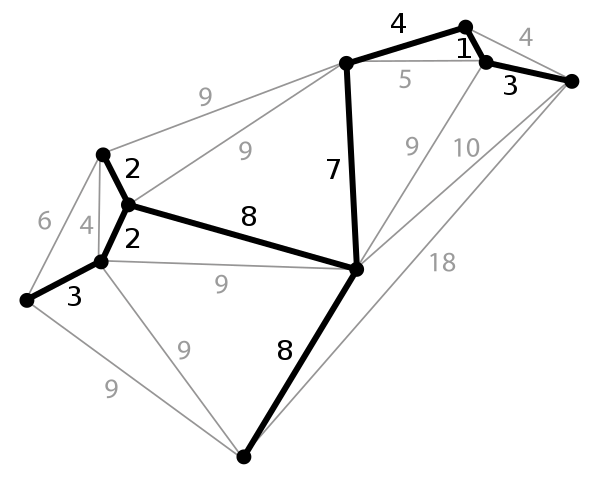
\includegraphics[scale=0.3]{images/tsp-msp}
			\caption{[Abb7] Traveling-Salesman-Problem}
		\end{figure}
	}
\end{frame}
  \begin{frame}
    \frametitle{Die Heuristik von Christofides - Schritt 2}
    Finde ein minimales perfektes Matching $M$ auf den Knoten von $T$ mit ungeradem Grad.
    \begin{itemize}
        \item Optimal: Blossom-Algorithmus, Linear Programming.
        \item Greedy-Algorithmus, $\mathcal{O}(|E'|\log |E'|) = \mathcal{O}(n^2\log n)$.
        \item $w(M) < \frac{1}{2}w(H_{\mathrm{opt}})$. %add graphic
    \end{itemize}
\end{frame}
  \begin{frame}
    \frametitle{Die Heuristik von Christofides - Schritt 3}
    Finde einen Eulerkreis $E$ auf $T \dot{\cup} M$.
    \begin{itemize}
        \item Bei uns: Algorithmus von Fleury $\mathcal{O}(|E_{T \dot{\cup} M}|^2) = \mathcal{O}(n^2)$.
        \item Alternativ: Algorithmus von Hierholzer $\mathcal{O(n)}$.
        \item $w(E) \leq w(T + M) = w(T) + w(M) < \frac{3}{2}w(H_{\mathrm{opt}})$.
    \end{itemize}
\end{frame}
  \begin{frame}
    \frametitle{Die Heuristik von Christofides - Schritt 4}
    Finde einen Hamiltonkreis $H$ aus $E$.
    \begin{itemize}
        \item Algorithmus: Überspringe alle bereits besuchten Knoten: $\mathcal{O}(n)$.
        \item $w(H) \leq w(E) < \frac{3}{2} w(H_{\mathrm{opt}})$.
    \end{itemize}
\end{frame}
  \begin{frame}
    \frametitle{Die Heuristik von Christofides}
    Als Ausgangsgraph betrachten wir $G = K_n$.
    \begin{enumerate}
        \item minimalen Spannbaum $T$ von $G$ 
        \item kostenminimales, perfektes Matching $M$ auf den Knoten von $T$ mit ungeradem Grad
        \item Eulerkreis $E$ auf $M \dot{\cup} T$
        \item Hamiltonkreis $H$ aus Eulerkreis $E$
    \end{enumerate}
\end{frame}
  \begin{frame}
	\frametitle{Weitere Optimierungen}
	\only<1,3,5> {
		\begin{itemize}
			\item<1->	$k$-opt-Verfahren.
			\item<3-> 	Ant-Colony-Optimization
			\item<5->	Andere Ansätze: Linear Programming
		\end{itemize}
	}

	\only<2> {
		\begin{figure}
			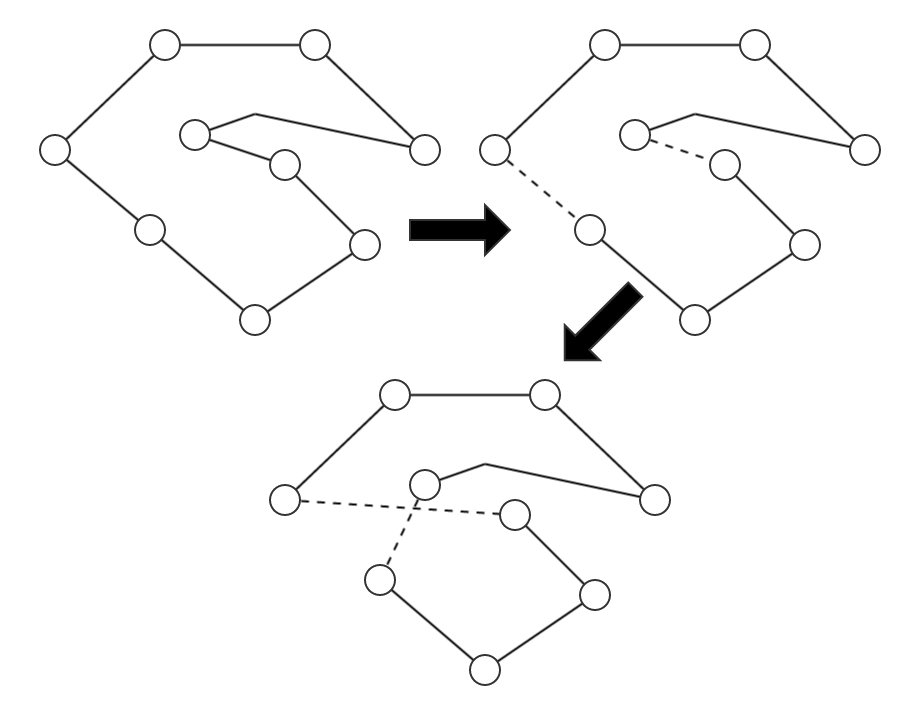
\includegraphics[scale=.2]{Showing_a_step_of_the_two-opt_heuristic.png}
			\caption{2-opt-Verfahren}
		\end{figure}
	}

	\only<4> 	{
		\begin{figure}
			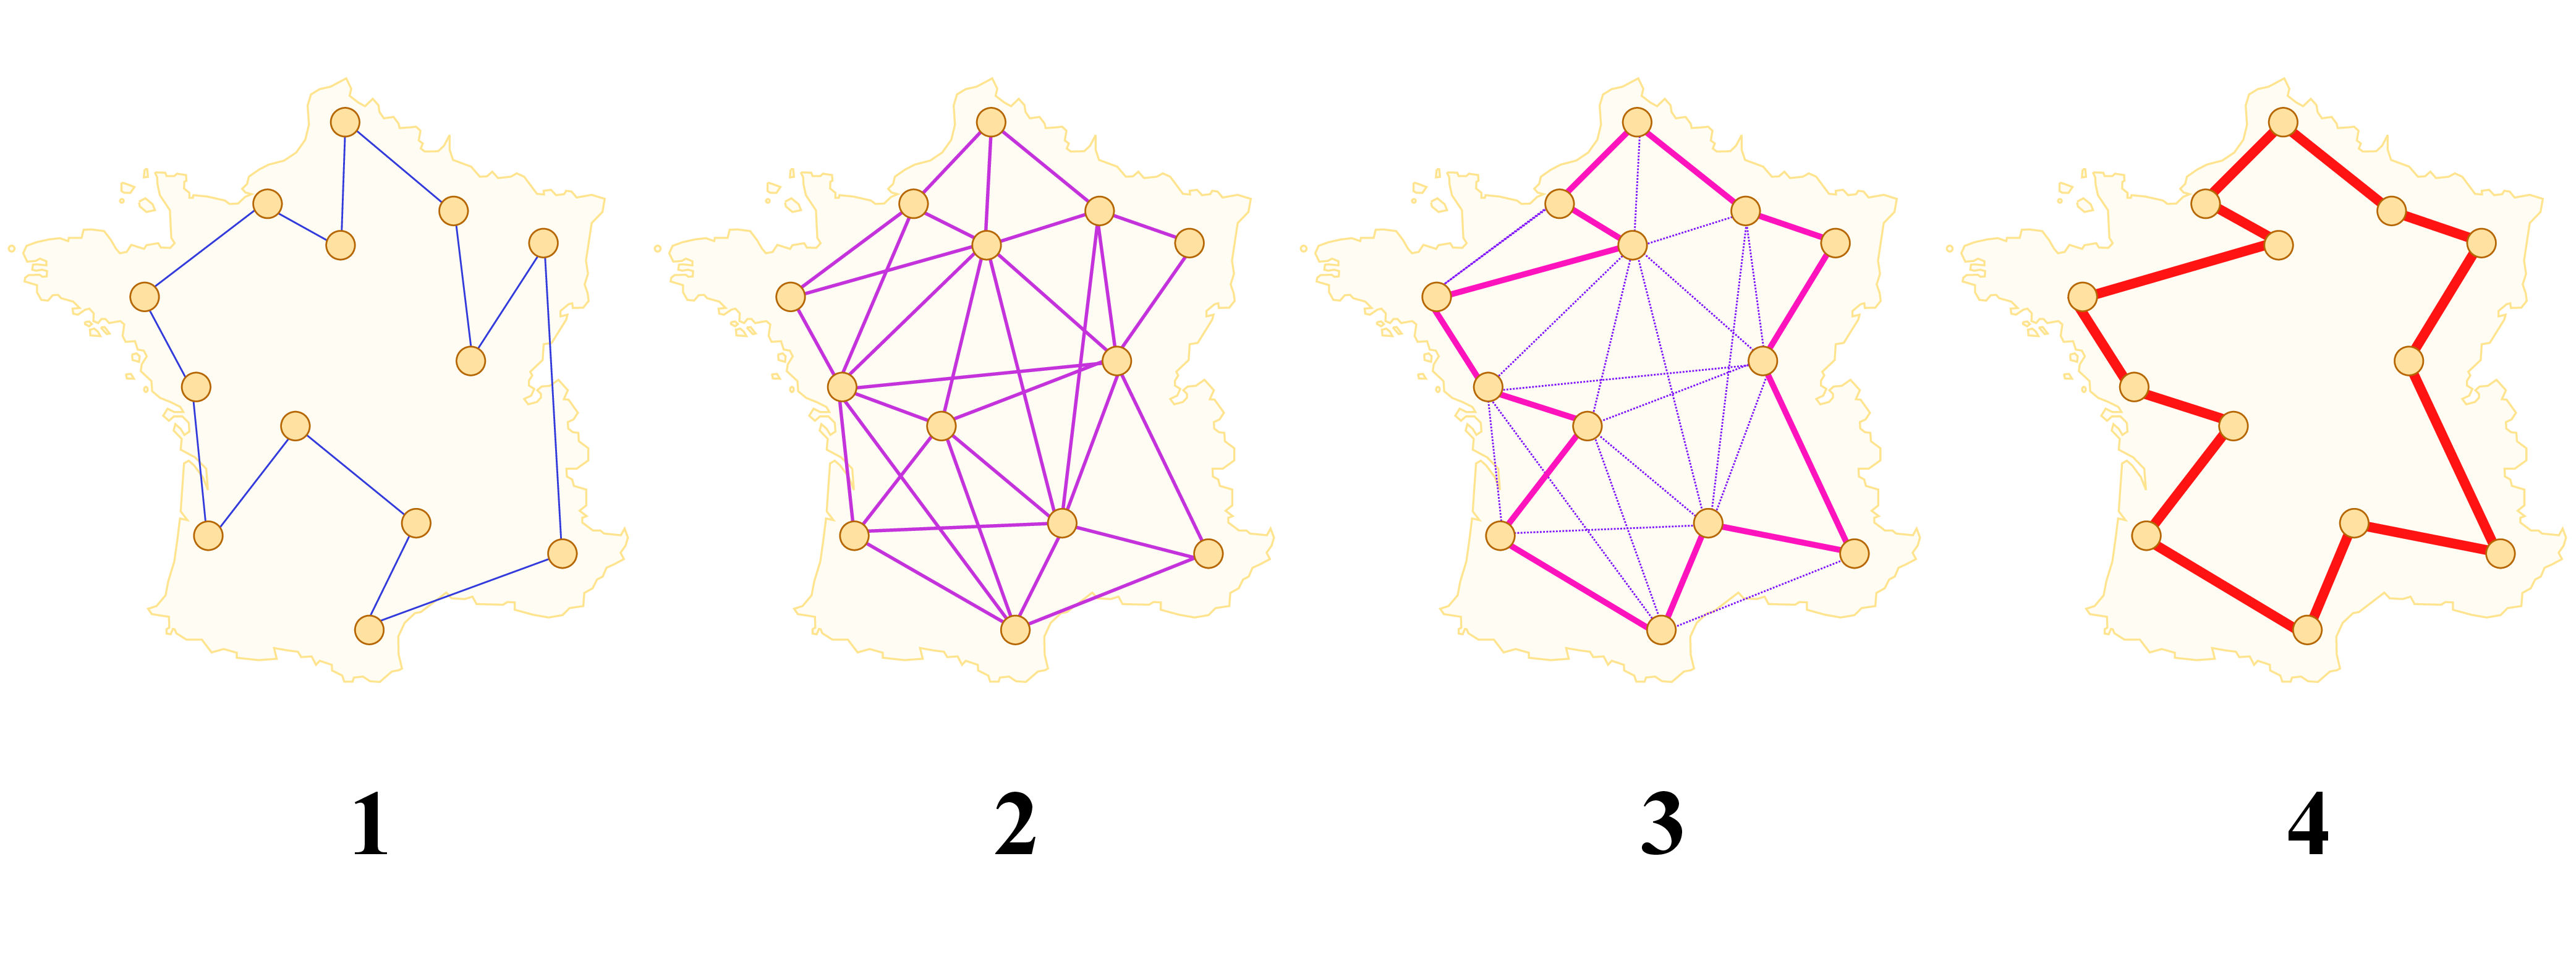
\includegraphics[scale=0.3]{images/traveling-salesman-problem}
			\caption{Die Dicke der Kanten ist proportional zu den Pheromonen, die darauf verteilt sind}
		\end{figure}
	}
\end{frame}
  \end{document}